\documentclass[11pt]{article}
\usepackage[margin=1in]{geometry}
\usepackage{amsmath,amssymb,amsthm}
\usepackage{tikz}
\usepackage{booktabs}
\usepackage{hyperref}
\usepackage{listings}
\lstset{basicstyle=\ttfamily\small,columns=fullflexible}

\newtheorem{theorem}{Theorem}
\newtheorem{lemma}[theorem]{Lemma}
\newtheorem{proposition}[theorem]{Proposition}
\theoremstyle{remark}
\newtheorem{remark}[theorem]{Remark}

\newcommand{\Con}{\operatorname{Con}}
\newcommand{\Eq}{\operatorname{Eq}}
\newcommand{\End}{\operatorname{End}}
\newcommand{\Cg}{\operatorname{Cg}}
\newcommand{\LL}{\mathbf{L}_7}

\title{DeMeo's exceptional seven-element lattice\\is the congruence lattice of a finite algebra}
\author{Bj{\o}rn Kjos-Hanssen}
\date{September 2026}

\begin{document}
\maketitle

\begin{abstract}
Let $\LL$ be the seven-element lattice singled out in W.~DeMeo's dissertation
\cite{DeMeo2012} as the smallest lattice not known to be isomorphic to the congruence
lattice of a finite algebra (it is the lattice $\mathbf L_{10}$ of the DeMeo--Freese
catalogue \cite{DeMeoFreese}). We show that $\LL$ is representable: it is the interval
$[H,G]$ in the subgroup lattice of $G=\mathrm{Sp}(6,2)$ for $H$ the normaliser of a Sylow
$7$-subgroup, of $G=\mathrm{PSL}(2,64)$ for $H\cong S_3$, of $G=\mathrm{McL}$ for
$|H|=120$, and of $G=\mathrm{Co}_3$ for $|H|=1440$; hence $\LL\cong\Con(G/H)$ for the
corresponding transitive $G$-sets, the smallest of which has $34\,560$ elements. The
$\mathrm{PSL}(2,64)$ example can be verified by hand from Dickson's list of subgroups.
The examples were found by scanning the GAP Library of Tables of Marks and confirmed by
independent computations. In the other direction, an exhaustive search over sublattices of the
partition lattice $\Eq(n)$ shows directly that $\LL\not\cong\Con\mathbf A$ for $|A|\le 13$,
and a search over all transitive permutation groups of degree at most $47$, using the theorem
of DeMeo and Freese that a minimal representation must be a transitive group, shows that
$\LL$ is not the congruence lattice of any algebra with at most $47$ elements. So the minimal
size of an algebra with congruence lattice $\LL$ lies between $48$ and $34\,560$.
\end{abstract}

\section{The lattice}

$\LL$ has elements $0,\,K,\,J_1,\,J_2,\,M_1,\,M_2,\,1$ with covering relations
\[
0\prec K\prec 1,\qquad 0\prec J_1\prec M_1\prec 1,\qquad 0\prec J_2\prec M_1,\qquad J_2\prec M_2\prec 1 .
\]
Thus $K,J_1,J_2$ are the atoms, $M_1=J_1\vee J_2$ and $M_2$ are the coatoms, $M_1\wedge M_2=J_2$,
$K\vee x=1$ for every $x\ne 0$, $J_1\vee M_2=1$, and $K\wedge x=0=J_1\wedge M_2$ for
$x\in\{J_1,J_2,M_1,M_2\}$. The atom $K$ is also a coatom, and $M_2$ is join-irreducible.
The lattice is self-dual and non-modular (it contains the pentagon $0<J_1<M_1<1$, $K$).
In the notation of the catalogue file \texttt{L10.tex} of \cite{DeMeoFreese}:
\emph{covers: bottom$<$wing, bottom$<$n11, bottom$<$11, wing$<$top, n11$<$02, 11$<$02, 11$<$22,
02$<$top, 22$<$top; represented-by: none known.}

\begin{center}
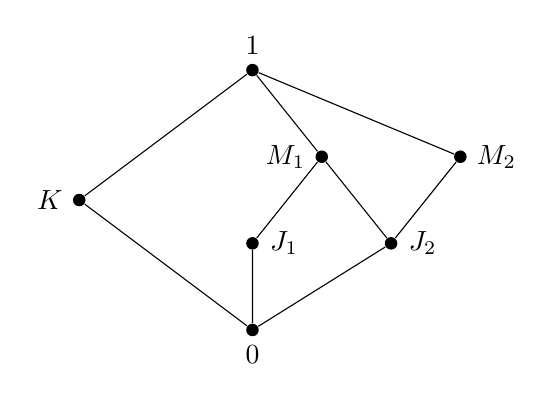
\begin{tikzpicture}[scale=1.1, every node/.style={circle,fill,inner sep=1.6pt}]
  \node (0) at (0,0) [label=below:$0$] {};
  \node (K) at (-2,1.5) [label=left:$K$] {};
  \node (J1) at (0,1) [label=right:$J_1$] {};
  \node (J2) at (1.6,1) [label=right:$J_2$] {};
  \node (M1) at (0.8,2) [label=left:$M_1$] {};
  \node (M2) at (2.4,2) [label=right:$M_2$] {};
  \node (1) at (0,3) [label=above:$1$] {};
  \draw (0)--(K)--(1); \draw (0)--(J1)--(M1)--(1); \draw (0)--(J2)--(M1); \draw (J2)--(M2)--(1);
\end{tikzpicture}
\end{center}

DeMeo \cite[Ch.~6]{DeMeo2012} showed that every other lattice with at most seven elements is
representable, and proved \cite[Thm.~4.1]{DeMeoIEP} that a representation of $\LL$ as an
interval $[H,G]$ in a subgroup lattice with $H$ core-free forces $G$ to be an
insoluble primitive permutation group. The representations found below are of exactly this kind.

\section{Representations}\label{sec:rep}

Recall (P\'alfy--Pudl\'ak \cite{PP}) that for a transitive $G$-set $G/H$ the congruence lattice
$\Con(G/H)$ is isomorphic to the interval $[H,G]$ in the subgroup lattice of $G$; the algebra
is $\langle G/H, (x\mapsto gx)_{g\in G}\rangle$, and two generators of $G$ suffice.

\begin{theorem}\label{thm:rep}
$\LL$ is isomorphic to the interval $[H,G]$ for each of the following pairs, and hence is the
congruence lattice of a finite algebra with $|G:H|$ elements.
\begin{center}
\begin{tabular}{llll}
\toprule
$G$ & $H$ & the five subgroups strictly between $H$ and $G$ & $|G:H|$\\
\midrule
$\mathrm{Sp}(6,2)$ & $7{:}6=N_G(P_7)$ & $L_3(2){:}2,\ L_2(8){:}3,\ S_7,\ U_3(3){:}2,\ S_8$ & $34\,560$\\
$\mathrm{PSL}(2,64)$ & $S_3$ & $D_{18},\ D_{42},\ A_5,\ D_{126},\ \mathrm{PSL}(2,8)$ & $43\,680$\\
$\mathrm{McL}$ & $3{:}(5{:}8)$, order $120$ & orders $720,\ 3000,\ 9720,\ 40320,\ 58320$ & $7\,484\,400$\\
$\mathrm{Co}_3$ & $\mathrm{SL}(2,5){:}D_{12}$, order $1440$ & orders $8640,\ 116640,\ 699840,\ 756000,\ 2903040$ & $344\,282\,400$\\
\bottomrule
\end{tabular}
\end{center}
In each case $H$ is self-normalising and core-free. The lattice elements are, in the order
$K,\ J_1,\ J_2,\ M_1,\ M_2$:
for $\mathrm{Sp}(6,2)$: $L_2(8){:}3,\ S_7,\ L_3(2){:}2,\ S_8,\ U_3(3){:}2$;
for $\mathrm{PSL}(2,64)$: $A_5,\ D_{42},\ D_{18},\ D_{126},\ \mathrm{PSL}(2,8)$;
for $\mathrm{McL}$: orders $3000,\ 9720,\ 720,\ 58320,\ 40320$;
for $\mathrm{Co}_3$: orders $756000,\ 116640,\ 8640,\ 699840,\ 2903040$.
The same interval occurs in $\mathrm{McL}{:}2$ (with $|H|=240$) and, lifted, in $2.\mathrm{Sp}(6,2)$.
\end{theorem}

\begin{proof}[Computer proof]
For each pair, \texttt{IntermediateSubgroups(G,H)} in GAP returns exactly five subgroups, and
the containment relation on the seven groups $H$, the five, $G$ (computed with
\texttt{IsSubgroup} for all $49$ pairs) is isomorphic to $\LL$; the isomorphism was found by
trying all $7!$ bijections. The files \texttt{L7\_in\_Sp6\_2.g}, \texttt{L7\_in\_L2\_64.g},
\texttt{L7\_in\_Co3.g} contain explicit permutation generators for $G$ and $H$ (on $63$, $65$
and $276$ points respectively; the $\mathrm{Co}_3$ generators are the ATLAS standard
generators) and the two-line check. For $\mathrm{Sp}(6,2)$ and $\mathrm{PSL}(2,64)$ the groups
were built from scratch (\texttt{Sp(6,2)}, \texttt{PSL(2,64)}): $\mathrm{Sp}(6,2)$ has a single
conjugacy class of subgroups of order $42$ and $\mathrm{PSL}(2,64)$ a single class of subgroups
of order $6$ (it has no elements of order $6$), so the choice of $H$ is forced.
\end{proof}

\begin{proposition}\label{prop:hand}
Let $G=\mathrm{PSL}(2,64)$ and $H\cong S_3$ a subgroup. Then $[H,G]\cong\LL$.
\end{proposition}
\begin{proof}
Write $q=64=2^6$, so $q-1=63=3^2\cdot 7$ and $q+1=65=5\cdot 13$. By Dickson's theorem the
subgroups of $G$ are: subgroups of the Borel subgroup $2^6{:}63$ (a Frobenius group with
kernel the Sylow $2$-subgroup); cyclic and dihedral groups $C_d$, $D_{2d}$ with $d\mid 63$ or
$d\mid 65$; and the subfield groups $\mathrm{PSL}(2,2^m)$, $m\mid 6$, i.e.\ $S_3$, $A_5$,
$\mathrm{PSL}(2,8)$, $G$ ($S_4$ does not occur since $8\nmid q\pm1$). A subgroup of order $6$
of the Borel subgroup meets the Frobenius kernel in a normal Sylow $2$-subgroup, so it is not
$S_3$; and $3\nmid 65$. Hence the subgroups containing $H$ are, up to conjugacy, among
$D_{18}, D_{42}, D_{126}$ (the $D_{2d}$ with $3\mid d\mid 63$), $A_5$ and $\mathrm{PSL}(2,8)$.

Let $C_3\le H$. Its centraliser is a torus $C_{63}$, and $N_G(C_{63})=D_{126}$ contains all
involutions inverting $C_3$; since $63$ is odd, $N_G(H)=H$. For $d\in\{9,21,63\}$ the group
$D_{2d}$ containing $H$ is unique: it is $\langle C_d,t\rangle$ for the unique $C_d$ with
$C_3\le C_d\le C_{63}$ and any involution $t\in H$. The number of conjugates of $A_5$
containing $H$ is $\frac{|G:A_5|\cdot 10}{|G:H|}=1$ ($A_5$ is maximal, hence self-normalising,
and contains $10$ subgroups $S_3$), and the number of conjugates of $\mathrm{PSL}(2,8)$
containing $H$ is $\frac{|G:\mathrm{PSL}(2,8)|\cdot 84}{|G:H|}=\frac{520\cdot 84}{43680}=1$
($\mathrm{PSL}(2,8)$ is maximal and contains $28$ subgroups $C_3$, each in $3$ subgroups $S_3$).
So $H$ has exactly five proper overgroups: $D_{18}$, $D_{42}$, $D_{126}$, $A_5$,
$\mathrm{PSL}(2,8)$. Among these, $D_{18},D_{42}<D_{126}$ and $D_{18}<\mathrm{PSL}(2,8)$
(the latter contains a $D_{18}\ge H$, which must be the unique one); there are no other
containments, by orders and because $\mathrm{PSL}(2,8)$ has no subgroup of order $42$ (its
dihedral subgroups have $d\mid 7$ or $d\mid 9$). This is the poset
$0<K,J_1,J_2;\ J_1,J_2<M_1;\ J_2<M_2;\ K,M_1,M_2<1$ with
$K=A_5$, $J_1=D_{42}$, $J_2=D_{18}$, $M_1=D_{126}$, $M_2=\mathrm{PSL}(2,8)$.
\end{proof}

\subsection*{How the examples were found}
For a finite group $G$ with table of marks $M$ (rows and columns indexed by conjugacy classes
of subgroups $K_1,\dots,K_r$, $M_{ij}=|\{gK_i : K_j\le gK_ig^{-1}\}|$), the number of conjugates
of $K_i$ containing a fixed $H=K_j$ is $M_{ij}/M_{ii}$. So the number of proper overgroups of
$H$ and the number of comparable pairs among them can be read off from the marks, and $\LL$ is
recognised by: exactly five proper overgroups, exactly three comparable pairs among them. The
program \texttt{l7tom.g} applied this test to every class $j$ of every one of the $414$ tables in
the GAP Library of Tables of Marks \cite{TomLib} (version 1.2.11; $S_{13}$ exceeded the time
limit and was skipped), yielding $86$ candidate pairs $(G,H)$. Since the pattern
``five overgroups, three comparable pairs'' with the degree sequence of $\LL$ forces the poset to
be $\LL$, the candidates were then verified group-theoretically as in the proof of
Theorem~\ref{thm:rep} (\texttt{l7tom\_verify.g}): six of the $86$ are $\LL$, namely the pairs in
Theorem~\ref{thm:rep} together with $\mathrm{McL}{:}2$ and $2.\mathrm{Sp}(6,2)$; the other $80$
have five overgroups but a different containment pattern. The $\mathrm{Co}_3$ example was
additionally reconstructed without the table of marks, from ATLAS standard generators, as
$H=K\cap M_1^{\,g}$ for suitable maximal subgroups $K\cong U_3(5){:}S_3$, $M_1$ of order
$699840$ and a double-coset representative $g$.

\section{Reduction to a finite closure test}

Fix a finite set $A$ with $|A|=n$ and let $\Eq(A)$ be the lattice of equivalence relations on $A$.
For a set $S\subseteq\Eq(A)$ let
\[
\End(S)=\{f\colon A\to A : (x,y)\in\theta\Rightarrow (f(x),f(y))\in\theta \text{ for all }\theta\in S\},
\]
a transformation monoid, and for a monoid $M$ of self-maps of $A$ let
$\Con(A,M)$ be the lattice of $M$-invariant equivalence relations.

\begin{lemma}\label{lem:unary}
For every algebra $\mathbf A$ on $A$, $\Con\mathbf A=\Con(A,\operatorname{Pol}_1\mathbf A)$.
Consequently a lattice $L$ is isomorphic to $\Con\mathbf A$ for some algebra on $A$ iff
$L\cong\Con(A,M)$ for some transformation monoid $M$ on $A$.
\end{lemma}
\begin{proof}
An equivalence is a congruence iff it is preserved by all unary polynomials; conversely
$\Con(A,M)=\Con(A,M)$ for the unary algebra $(A,M)$.
\end{proof}

\begin{lemma}\label{lem:closure}
Let $S\subseteq\Eq(A)$ contain the equality and the full relation and be closed under
finite meets and joins in $\Eq(A)$. The following are equivalent:
\begin{enumerate}
\item[(i)] $S=\Con(A,M)$ for some transformation monoid $M$;
\item[(ii)] $S=\Con(A,\End(S))$;
\item[(iii)] for all $a\ne b$ in $A$, the equivalence relation $\Cg(a,b)$ generated by
$\{(f(a),f(b)) : f\in\End(S)\}$ equals the least element $\theta_{ab}$ of $S$ containing $(a,b)$.
\end{enumerate}
\end{lemma}
\begin{proof}
(i)$\Rightarrow$(ii): $M\subseteq\End(S)$ gives $S\subseteq\Con(A,\End(S))\subseteq\Con(A,M)=S$.
(ii)$\Rightarrow$(i) is trivial. For (ii)$\Leftrightarrow$(iii): $\Cg(a,b)$ is the principal
congruence of the unary algebra $(A,\End(S))$ generated by $(a,b)$, every congruence is a join
of principal ones, and $S$ is join-closed; moreover $\theta_{ab}\in S$ is $\End(S)$-invariant,
so $\Cg(a,b)\subseteq\theta_{ab}$ always, with equality for all pairs iff every principal
congruence lies in $S$, iff $\Con(A,\End(S))\subseteq S$.
\end{proof}

Hence $\LL\cong\Con\mathbf A$ for some $\mathbf A$ with $|A|=n$ iff some $\{0,1\}$-sublattice
$S\le\Eq(n)$ with $S\cong\LL$ satisfies condition (iii). Since $\operatorname{Sym}(n)$ acts on
$\Eq(n)$ by lattice automorphisms preserving everything in sight, the element of $S$
playing the role of $K$ may be taken to be a fixed representative of its
$\operatorname{Sym}(n)$-orbit, i.e.\ one partition for each multiset of block sizes.

\section{The search}

For each $n\le 12$ the program (\texttt{l7search.c}, later \texttt{l7sym.c}) enumerates all such $S$ as follows.
Equivalence relations are stored as canonical block-label vectors and as bitmasks over the
$\binom n2$ pairs, so that $\theta\wedge\theta'=0$ is a single bitwise AND.
For each canonical $K$ it forms the list $L_K$ of partitions $J$ with $K\wedge J=0$ and $K\vee J=1$;
then $J_1,J_2\in L_K$ range over ordered pairs with $J_1\wedge J_2=0$, $M_1:=J_1\vee J_2\ne 1$ and
$K\wedge M_1=0$. Finally $M_2$ is generated directly as a proper coarsening of $J_2$ whose pairs
avoid the forbidden set $\operatorname{pairs}(K)\cup\operatorname{pairs}(J_1)\cup
(\operatorname{pairs}(M_1)\setminus\operatorname{pairs}(J_2))$
(this is equivalent to $M_2\wedge K=0$, $M_2\wedge J_1=0$, $M_1\wedge M_2=J_2$), subject to
$K\vee M_2=1=J_1\vee M_2$. Every such $S=\{0,K,J_1,J_2,M_1,M_2,1\}$ is a $\{0,1\}$-sublattice
of $\Eq(n)$ isomorphic to $\LL$, and every such sublattice with $K$ canonical arises exactly once.
For each $S$ the monoid $\End(S)$ is enumerated by backtracking over the values
$f(0),f(1),\dots$ with the invariance constraints checked incrementally, and condition (iii)
is tested with early termination: the search of $\End(S)$ aborts as soon as some
$(f(a),f(b))$ leaves $\theta_{ab}$.

\paragraph{Symmetry reduction.} Let $\operatorname{Stab}(K)\le\operatorname{Sym}(n)$ be the
stabiliser of the partition $K$ and let $G'\subseteq\operatorname{Stab}(K)$ be any subset
(\texttt{l7sym.c} enumerates up to $60\,000$ elements). Restrict $J_1$ to those elements of $L_K$
that are lexicographically minimal, as canonical label vectors, among their images under $G'$.
This is sound for any subset $G'$: if $S$ is a candidate then so is $g(S)$ for $g\in\operatorname{Stab}(K)$,
with the same closure status, and the lexicographically least element of the
$\operatorname{Stab}(K)$-orbit of $J_1$ is in particular $G'$-minimal, so every orbit of candidates
is still represented. The reduction factor is close to $|G'|$. The implementation was checked
by recomputing the unreduced counts: for $n\le 9$ (where the full stabiliser is enumerated)
$\sum_{J_1\text{ minimal}}|\operatorname{Orb}(J_1)|\cdot c(J_1)$, with $c(J_1)$ the number of
completions $(J_2,M_2)$, reproduces $528$, $23\,664$ and $522\,192$ exactly.

\begin{center}
\begin{tabular}{rrrrr}
\toprule
$n$ & $|\Eq(n)|$ & $\{0,1\}$-sublattices $\cong\LL$ ($K$ canonical) & reduced ($J_1$ minimal) & closed\\
\midrule
$\le 5$ & $\le 52$ & 0 & 0 & 0\\
6 & 203 & 72 & 5 & 0\\
7 & 877 & 528 & 20 & 0\\
8 & 4\,140 & 23\,664 & 253 & 0\\
9 & 21\,147 & 522\,192 & 3\,153 & 0\\
10 & 115\,975 & 21\,162\,480 & 52\,159 & 0\\
11 & 678\,570 & 677\,466\,192 & 839\,079 & 0\\
12 & 4\,213\,597 & --- & 17\,907\,745 & 0\\
13 & 27\,644\,437 & --- & 386\,326\,679 & 0\\
\bottomrule
\end{tabular}
\end{center}

\begin{theorem}\label{thm:brute}
$\LL$ is not isomorphic to the congruence lattice of any algebra with at most $13$ elements.
\end{theorem}

The $n=13$ run was carried out on an Apple M5 with eight workers in about five hours.

\section{Transitive groups of degree up to 47}

DeMeo and Freese \cite[Section on intransitive group actions]{DeMeoFreese} prove: if
$L\cong\Con\langle A,F\rangle$ is a representation of minimal size and $L$ is simple and its
coatoms meet to $0$, then by P\'alfy--Pudl\'ak and McKenzie every nonconstant operation in $F$ is
a permutation, so $\Con\langle A,F\rangle=\Con\langle A,G\rangle$ for the group $G$ these
permutations generate; and they show, using their structure theorem for congruence lattices of
intransitive $G$-sets, that for $\mathbf L_{10}=\LL$ the group $G$ must be transitive.
Both hypotheses hold for $\LL$: it has only the two trivial lattice congruences (checked by
enumerating all $877$ equivalence relations on its seven elements), and its coatoms $K,M_1,M_2$
meet to $0$. For a transitive $G$-set the congruences are the block systems, which correspond to
the subgroups between the point stabiliser $G_a$ and $G$; so
\[
\text{$\LL$ has a representation of minimal size $n$}\iff
\text{$\LL\cong[G_a,G]$ for some transitive group $G$ of degree $n$.}
\]
GAP's TransGrp library \cite{TransGrp} contains every transitive group of degree at most $47$ up to
permutation isomorphism (degree $32$, with $2\,801\,324$ groups, is a separate download; it was
run (\texttt{l7trans32.g}) in about $35$ minutes). For each group $G$ the program
\texttt{l7trans.g} computes the blocks through the point $1$ of all nontrivial block systems
(\texttt{AllBlocks}), and when there are exactly five of them tests whether their inclusion
poset is that of $K,J_1,J_2,M_1,M_2$: exactly three strict inclusions, $J_1,J_2\subset M_1$ and
$J_2\subset M_2$. The correspondence between block systems and overgroups of $G_1$ was
verified on all $461$ transitive groups of degrees $6$--$12$ by comparing with
\texttt{IntermediateSubgroups}. The result:

\begin{center}
\begin{tabular}{rrrr}
\toprule
degree & transitive groups & with exactly 5 block systems & block lattice $\cong\LL$\\
\midrule
4--23 & 4\,949 & 595 & 0\\
24 & 25\,000 & 4\,868 & 0\\
25--31 & 10\,285 & 394 & 0\\
32 & 2\,801\,324 & 8\,886 & 0\\
33--39 & 122\,356 & 16\,781 & 0\\
40 & 315\,842 & 162\,416 & 0\\
41--47 & 22\,609 & 770 & 0\\
\bottomrule
\end{tabular}
\end{center}

\begin{theorem}\label{thm:trans}
$\LL$ is not isomorphic to the congruence lattice of any algebra with at most $47$ elements.
The minimal size of an algebra with congruence lattice $\LL$ lies between $48$ and $34\,560$,
and a minimal representation is a transitive permutation group of degree at least $48$.
\end{theorem}
\begin{proof}
If $\LL\cong\Con\mathbf A$ with $|A|=n$ minimal, then by the DeMeo--Freese theorem $\LL$ is the
block lattice of a transitive group of degree $n$; the table excludes every $n\le 47$. The upper
bound is the $\mathrm{Sp}(6,2)$-set of Theorem~\ref{thm:rep}.
\end{proof}

Theorem~\ref{thm:brute} is independent of this reduction and confirms it for $n\le 13$.
The transitive groups of degree $48$ ($195\,826\,352$ of them) are also available for GAP but
were not checked. The representations of Theorem~\ref{thm:rep} are primitive, in agreement with
DeMeo's theorem \cite[Thm.~4.1]{DeMeoIEP}; a minimal representation need not be primitive.

\section{Validation}

Two independent implementations were written: \texttt{l7search.c}, specialised to $\LL$ as
above, and \texttt{latrep.c}, which accepts an arbitrary finite lattice given by its covering
relations, enumerates meet- and join-preserving injections into $\Eq(n)$ by backtracking, and applies
the same closure test. The two agree on the counts in the table for $n=6,7,8$ (the generic
program was not run for $n\ge 9$). The generic program was checked against known minimal
representations: it finds $N_5$ first at $n=4$, $M_3$ at $n=3$, and the catalogue lattices
$\mathbf L_6$ and $\mathbf L_7$ of \cite{DeMeoFreese} exactly at $n=6$ and not below, as stated
there; and it reports no representation of $\mathbf L_9$ of \cite{DeMeoFreese} for $n\le 7$,
consistent with the catalogue's 16-element representation. As a further check, the closure
test was verified in Python on a small example by enumerating all $n^n$ maps directly.

\begin{remark}
The candidate counts grow by a factor of roughly $22$--$32$ per step in $n$, and the enumeration of
$\End(S)$ grows with $n$ as well; $n=10$ took about 15 minutes and $n=11$ about 14 hours on two
cores (the $n=11$ run was checkpointed per block and per range of $J_1$; the per-block counts are
summed from the checkpoint file). Only 18 of the 54 nontrivial block types of $K$ admit any
candidate at all, and two of them---$K$ of type $3+2+2+2+2$ and $3+3+3+2$---account for
$228$ and $249$ million candidates respectively. Pushing to $n=12$ ($|\Eq(12)|=4\,213\,597$)
would need the pair masks widened to 66 bits and, extrapolating, some $2\times 10^{10}$ candidates;
with the symmetry reduction it took 35 minutes on two cores ($17.9$ million reduced candidates
over the 75 block types, the largest contributions coming from $K$ of type $3+2+2+2+2+1$ and $4+3+3+2$).
The reduced search for $n=13$ ($|\Eq(13)|=27\,644\,437$, about $1.7$\,GB per worker) is estimated
at some tens of core-hours.
\end{remark}

\section*{Code}

\texttt{L7\_in\_Sp6\_2.g}, \texttt{L7\_in\_L2\_64.g} and \texttt{L7\_in\_Co3.g} each define $G$ and $H$
by explicit permutations and verify Theorem~\ref{thm:rep} in a few seconds (a few minutes for
$\mathrm{Co}_3$); \texttt{l7tom.g} with \texttt{l7tom\_driver.sh} and \texttt{l7tom\_verify.g} perform
the table-of-marks search; \texttt{l7trans.g} and \texttt{l7trans32.g} the transitive-group search.
\texttt{l7sym.c} with the driver \texttt{run\_sym.sh} (symmetry-reduced, parallel, checkpointed search,
$n\le 13$), the unreduced \texttt{l7search\_m5.c}, and \texttt{latrep.c} (generic lattice, $n\le 8$)
accompany this note. Usage: \texttt{./run\_sym.sh 12 8} runs the $n=12$ search on eight cores; \texttt{./latrep 6 "0<1 0<2 1<3 2<4 3<4"} tests $N_5$ at $n=6$.

\section*{Acknowledgments}
	Computations carried out with Claude (Anthropic).

\begin{thebibliography}{9}
\bibitem{DeMeo2012} W.~DeMeo, \emph{Congruence lattices of finite algebras}, Ph.D.\ thesis,
University of Hawaii at M\=anoa, 2012; arXiv:1204.4305.
\bibitem{DeMeoIEP} W.~DeMeo, \emph{Interval enforceable properties of finite groups},
arXiv:1205.1927.
\bibitem{DeMeoFreese} W.~DeMeo and R.~Freese, \emph{Representing finite lattices as congruence
lattices of finite algebras}, \url{https://github.com/UniversalAlgebra/fin-lat-rep}.
\bibitem{TomLib} T.~Merkwitz, L.~Naughton and G.~Pfeiffer, \emph{TomLib, the GAP library of tables of marks},
GAP package, version 1.2.11.
\bibitem{TransGrp} A.~Hulpke, \emph{TransGrp, transitive groups library}, GAP package, version 3.6.5;
data by Butler, Conway, Hulpke, Holt, Royle and others.
\bibitem{PP} P.~P.\ P\'alfy and P.~Pudl\'ak, Congruence lattices of finite algebras and intervals
in subgroup lattices of finite groups, Algebra Universalis 11 (1980), 22--27.
\end{thebibliography}
\end{document}
